% CHAPTER 1
\chapter{POWER SYSTEM FREQUENCY STABILITY}
\label{chp:2}

\section{Frequency in a Power System}
\subsection{Synchronous Generator and Synchronous Speed}

Synchronous machines produce torque only in synchronous speed. This is why they are equipped with damper windings which are basically induction machine windings. If the frequency of  grid changes, damper windings create a torque which creates a force to synchronize the speed to the grid frequency. Two type of damper windings are given in Figure \ref{damperwindings}.

\begin{figure}[h!]
	\centering
	\begin{subfigure}{.5\textwidth}
		\centering
		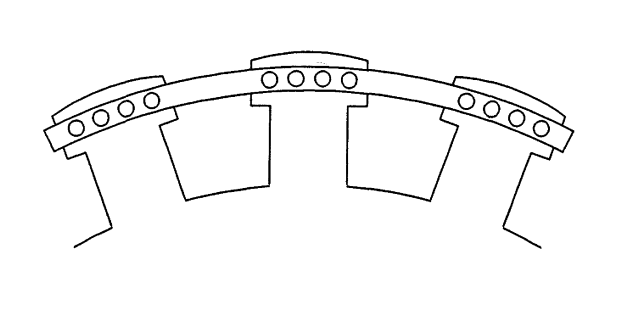
\includegraphics[width=.95\linewidth]{continuousdamper.png}
		\caption{continuous damper}
		\label{continuousdamper}
	\end{subfigure}%
	\begin{subfigure}{.5\textwidth}
		\centering
		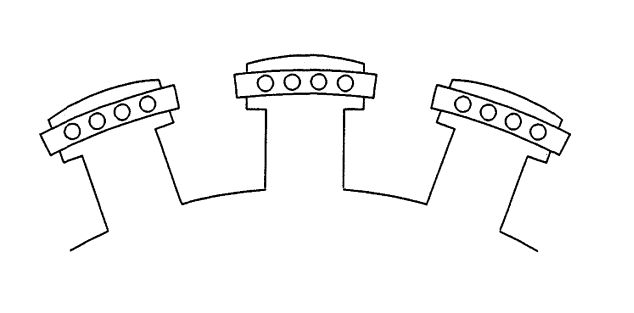
\includegraphics[width=.95\linewidth]{noncontinuousdamper.png}
		\caption{non-continuous damper}
		\label{noncontinuousdamper}
	\end{subfigure}
	\caption{Damper windings in a synchronous generator \cite{Kundur}}
	\label{damperwindings}
\end{figure}

Due to the damper windings in the rotor, the synchronous machines always operate in synchronous speed. Relation between grid frequency and the synchronous speed is given in \ref{syncspeed}

\begin{equation}
 n_{s}=\frac{120f}{p_{f}}\cite{Kundur}
\end{equation}
\begin{equation}
 n_{s}=\frac{60}{2\pi}\omega_{syn}
\end{equation}
\begin{equation}
\omega_{syn}=\frac{4\pi f}{p_{f}}
\label{syncspeed}
\end{equation}

where $n_{s}$ is the synchronous speed in rpm, $f$ is the grid frequency in Hz, $p_{f}$ is the number of poles of the corresponding generator and $\omega_{syn}$ is the synchronous angular speed in rad/s.

\subsection{Swing Equation}
Speed in synchronous machines changes according to the net torque acting on the rotor. Therefore, the speed is maintained constant unless there is no difference between mechanical and electromechanical torque. The equation of motion is given in Eq.\ref{eqmotion} where $J$ is aggravated moment of inertia of the generator and the turbine in $kgm^{2}$,$T_{m}$ and $T_{e}$ are mechanical and electromechanical torques in $Nm$.

\begin{equation}
J\frac{d\omega_{m}}{dt}=T_{m}-T_{e}=T_{a}
\label{eqmotion}
\end{equation}

In power system network, the power ratings of the generators and corresponding moment of inertia values varies. Hence, it is more convenient to use inertia constant, $H$ whose unit is seconds and varies between 2 and 9. Inertia constant is defined as the ratio of kinetic energy stored in the inertia to the power rating of the generator as in Eq.\ref{inertiaconstant} where $\omega_{0m}$ denotes the rated angular velocity of generator in rad/s and $S_{base}$ is the rated apparent power in VA. 
\begin{equation}
H=\frac{{\frac{1}{2}}J\omega_{0m}^{2}}{S_{base}}
\label{inertiaconstant}
\end{equation}

Substituting Eq.\ref{inertiaconstant} into Eq.\ref{eqmotion} and replacing units to per-unit quantities yield the relation of frequency with power and inertia constant as in Eq.\ref{eqmotion5}

\begin{equation}
J=\frac{2H}{\omega_{0m}^{2}}{S_{base}}
\label{inertiaconstant2}
\end{equation}

\begin{equation}
\frac{2H}{\omega_{0m}^{2}}{S_{base}}\frac{d\omega_{m}}{dt}=T_{m}-T_{e}
\label{eqmotion2}
\end{equation}

\begin{equation}
\frac{2H}{\omega_{0m}^{2}}{S_{base}\omega_{m}}\frac{d\omega_{m}}{dt}=P_{m}-P_{e}
\label{eqmotion3}
\end{equation}

\begin{equation}
2H\frac{\omega_{m}}{\omega_{0m}}\frac{d(\omega_{m}/\omega_{0m})}{dt}=\frac{P_{m}-P_{e}}{S_{base}}
\label{eqmotion4}
\end{equation}

\begin{equation}
2H\overline{\omega_{m}}\frac{d\overline{\omega_{m}}}{dt}=\overline{P_{m}}-\overline{P_{e}}
\label{eqmotion5}
\end{equation}

\subsection{Frequency in Power Systems}
